% !TEX root = ../main.tex
%
\chapter{Results}
\label{sec:result}

This section presents the results of the user study conducted to evaluate the usability of the application.
First the results of the quantitative user experience questionnaire are presented, to gauge the overall user experience.
Then the results of the qualitative user testing are presented, to provide more detailed insights into the user experience.
Finally, the results are integrated and discussed.

\section{User Experience Questionnaire}
\label{sec:result:ux}

Even with the relatively small sample size of 10 participants, the results of the User Experience Questionnaire (UEQ) provide a good overview of the overall user experience.
The scores for the different scales of the UEQ are shown in Figure~\ref{fig:ueq-1}. 
The \emph{Novelty} scale has the lowest score with 1.4 and the \emph{Attractiveness} scale has the highest score with 2.0.

\begin{figure}[htb]
	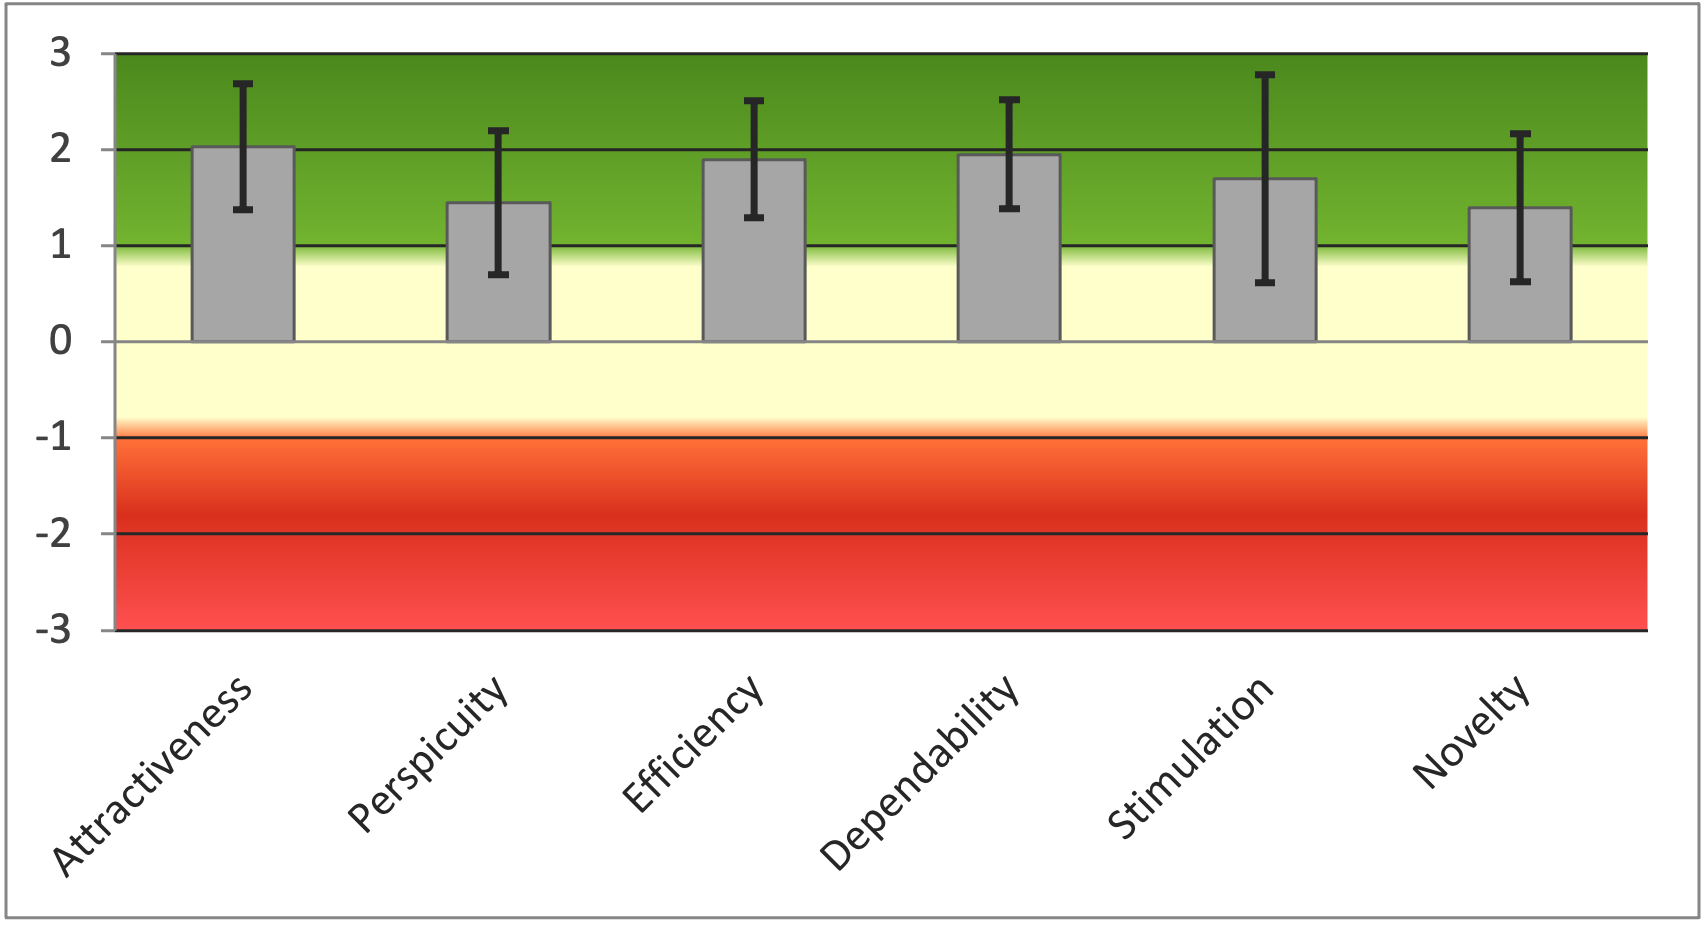
\includegraphics[width=\textwidth]{figures/ueq-1.png}
	\caption{Results of the User Experience Questionnaire}
  \label{fig:ueq-1}
\end{figure}

These results show that the application is generally well received by the participants.

The UEQ provides a benchmark containing the results of 452 other studies. 
The benchmarking results of the UEQ are shown in Figure~\ref{fig:ueq-2}.
Three out of the six scales classify as \emph{Excellent}, placing them in the top 10\% of all studies.
Comparatively low scores are achieved in the scales \emph{Perspicuity} 

\begin{figure}[htb]
	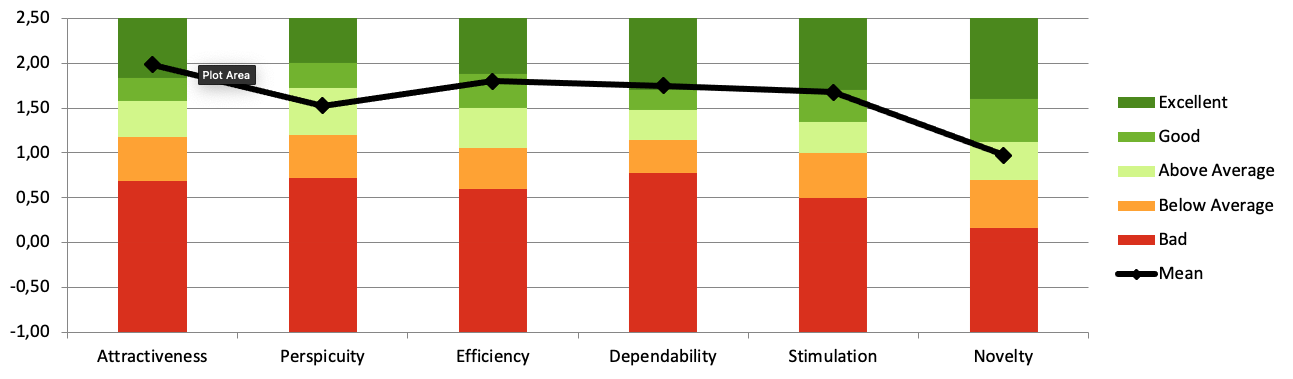
\includegraphics[width=\textwidth]{figures/ueq-2.png}
  \caption{Benchmarking Results of the User Experience Questionnaire}
  \label{fig:ueq-2}
\end{figure}

\section{Findings from Qualitative User Testing}
\label{sec:result:testing}


\section{Integration and Findings}
\label{sec:result:findings}

